\chapter{\acs{lidar} Interference}
\label{chapter:lidar-interference}

\ac{lidar} interference is occurs when the signal of one \ac{lidar}, ``A'', interferes with the signal of another \ac{lidar}, ``B'', affecting its measurements, i.e., the \ac{lidar}'s ``B'' capability to measure the distance what which is laser pulse was reflected is not independent of the presence of another \ac{lidar} on its surroundings. On telecommunications, when two devices on the same channel or physical environment interact, creating an undesirable effect with negative consequences, we are in the presence of crosstalk. On the \ac{lidar} interference scenario, this interference can be direct or indirect (the beam is reflected on other surface(s) before hitting the \ac{lidar} ``B'').

The main goal of this thesis is to research the \ac{lidar}'s interference behavior, expanding the previous work, presented on the Section~\ref{sec:sota:lidar-interference}. \acl{sota} on \ac{lidar} interference is still reduced, with the major contributions from only two research teams, and for an experimental setup with only two-dimensional \acp{lidar}, i.e., rotating \acp{lidar} that can scan a single line from the environment.

On this chapter, we start by explaining the additions to the previously described experimental setup, on Section~\ref{sec:calibration:experimental-setup}, that allows us to investigate the impact of several parameters on \ac{lidar} interference behavior. Experimental test scenarios are detailed and the test conditions under which data was acquired are explained. Since one of the thesis objectives, detailed in Section~\ref{sec:introduction:objectives}, is to create a comprehensive experimental dataset, with different metrics, for future tests on \ac{lidar} interference, we present how the experimental dataset was organized to ensure it could be easily reused but also to streamline data analysis on this research.

Our first \ac{lidar} interference analysis results are obtained from Bosch\cp~datasets, allowing a qualitative assessment of the interference. Based on these results, we sought to explain this behavior by quantifying the number of outliers that have no physical context on the data, such as points below ground or outside a closed room dimensions.

To provide a more in-depth analysis of the interference, a comparison with a ground-truth model of the test environment is required. Therefore, we propose two methods to generate such ground truth model from the data without interference. Using these models, we also propose two methods to measure the interference, unveiling their algorithms and results.

Following up on the outcomes provided by Chapter~\ref{chapter:object-detection}, we apply the previous algorithms onto the selected \acp{roi} on the point cloud, that correspond to the bounding boxes of image objects previously detected on the image, using the calibration notions gathered from Chapter~\ref{chapter:calibration}.

Lastly, we conclude our findings and compare them with the current \acl{sota} on \ac{lidar} interference.

\section{Experimental Setup}
\label{sec:lidar-interference:experimental-setup}

Expanding the previous experimental setup, detailed in Section~\ref{sec:calibration:experimental-setup}, requires adding another \ac{lidar}, that acts as an interferer. This \ac{lidar} is mounted on a tripod and serves the purpose of interfering with the measurements of the first \ac{lidar}, already present on the earlier version of the experimental setup (see figure~\ref{fig:experimental-setup}), which becomes its ``victim''\footnote{The terms victim and interferer, when referring to \ac{lidar} interference, are first connoted by Gunzung Kim\etal on~\cite{Kim2015a, Kim2015b, Kim2015c, Kim2017}, and later adopted by Gerald Popko\etal~\cite{Popko2019a, Popko2019b}. To keep the notation coherent with the \acl{sota}, we will use the same denominations on this chapter.}.

The interferer \ac{lidar} is a HESAI\cp~Pandar40\texttrademark, a 40 beams \ac{tof} \ac{lidar} that operates at a frequency of \SI{905}{\nano\meter}. Pandar40 supports various measurements modes based on the return pulse (Strongest, Last, Dual) and can be connected to a \ac{gps} receiver for geopositioning and synchronization with an external clock. It also supports two rotation velocities: 600 or 1200 \ac{rpm}, which result in different angular steps and point cloud refresh rate. 

Pandar40's \ac{lidar} has an asymmetrical vertical \ac{fov}, varying from \SIrange{-16}{+7}{\degree}. A larger channel density occurs between the angles \SI{-6}{\degree} and \SI{+2}{\degree}, with 25 pairs of lasers and photoreceptors with \SI{0.33}{\degree} apart from each other. From \SIrange{-16}{-6}{\degree} and \SIrange{+2}{+7}{\degree}, the angular step between the pairs of lasers and photoreceptors is \SI{1}{\degree}, and only 15 pairs of lasers and photoreceptors are used: 5 above and 10 below.

The full specifications of the HESAI Pandar40 can be accessed on~\cite{Pandar40UserGuide} and the relevant specifications for this work are summarized on table~\ref{tab:pandar40-specs}.

\begin{table}[H]
	\centering
	\renewcommand{\arraystretch}{1.2}
	\rowcolors{3}{gray!10}{white}
	\begin{tabular}{@{}p{6cm}c@{}}
		\toprule
		Specifications & Value \\
		\midrule
		Wavelength & \SI{905}{\nano\meter} \\
		Motor \ac{rpm} & 600 \\
		Angular Step & \SI{0.2}{\degree} \\
		Vertical \ac{fov} & \SI{23}{\degree} \\
		Horizontal \ac{fov} & \SI{360}{\degree} \\
		Maximum Scanning Distance & \SI{200}{\meter} @20\% reflectivity \\
																					 & $\pm \SI{5}{\centi\meter}$, from \SIrange{0.3}{0.5}{\meter} \\
		\rowcolor{white} \multirow{-2}{*}{Measurement Accuracy} & $\pm \SI{2}{\centi\meter}$, from \SIrange{0.5}{200}{\meter} \\
		\bottomrule
	\end{tabular}
	\caption{HESAI Pandar40 relevant specifications. Source~\cite{Pandar40UserGuide}.}
	\label{tab:pandar40-specs}
\end{table}

The tripod used for the experimental setup is a Velbon\cp~CX-460\texttrademark~tripod, that also has a central monopod. For increased stability on the measurement procedure, the monopod was never used. The tripod ranges in height from approximately \SIrange{0.62}{1.28}{\meter}, measured from its feet to its basis. Since the tripod used is a camera tripod, a gimmick must be done to ensure proper fixation of the Pandar40 \ac{lidar}, by replacing the universal camera support bolt with an \SI{12}{\milli\meter} length M6 bolt, tighten with a M6 nut and two metal rings. The Pandar40, secured on the tripod, is shown on figure~\ref{fig:pandar40-on-tripod}.

\begin{figure}[H]
	\centering
	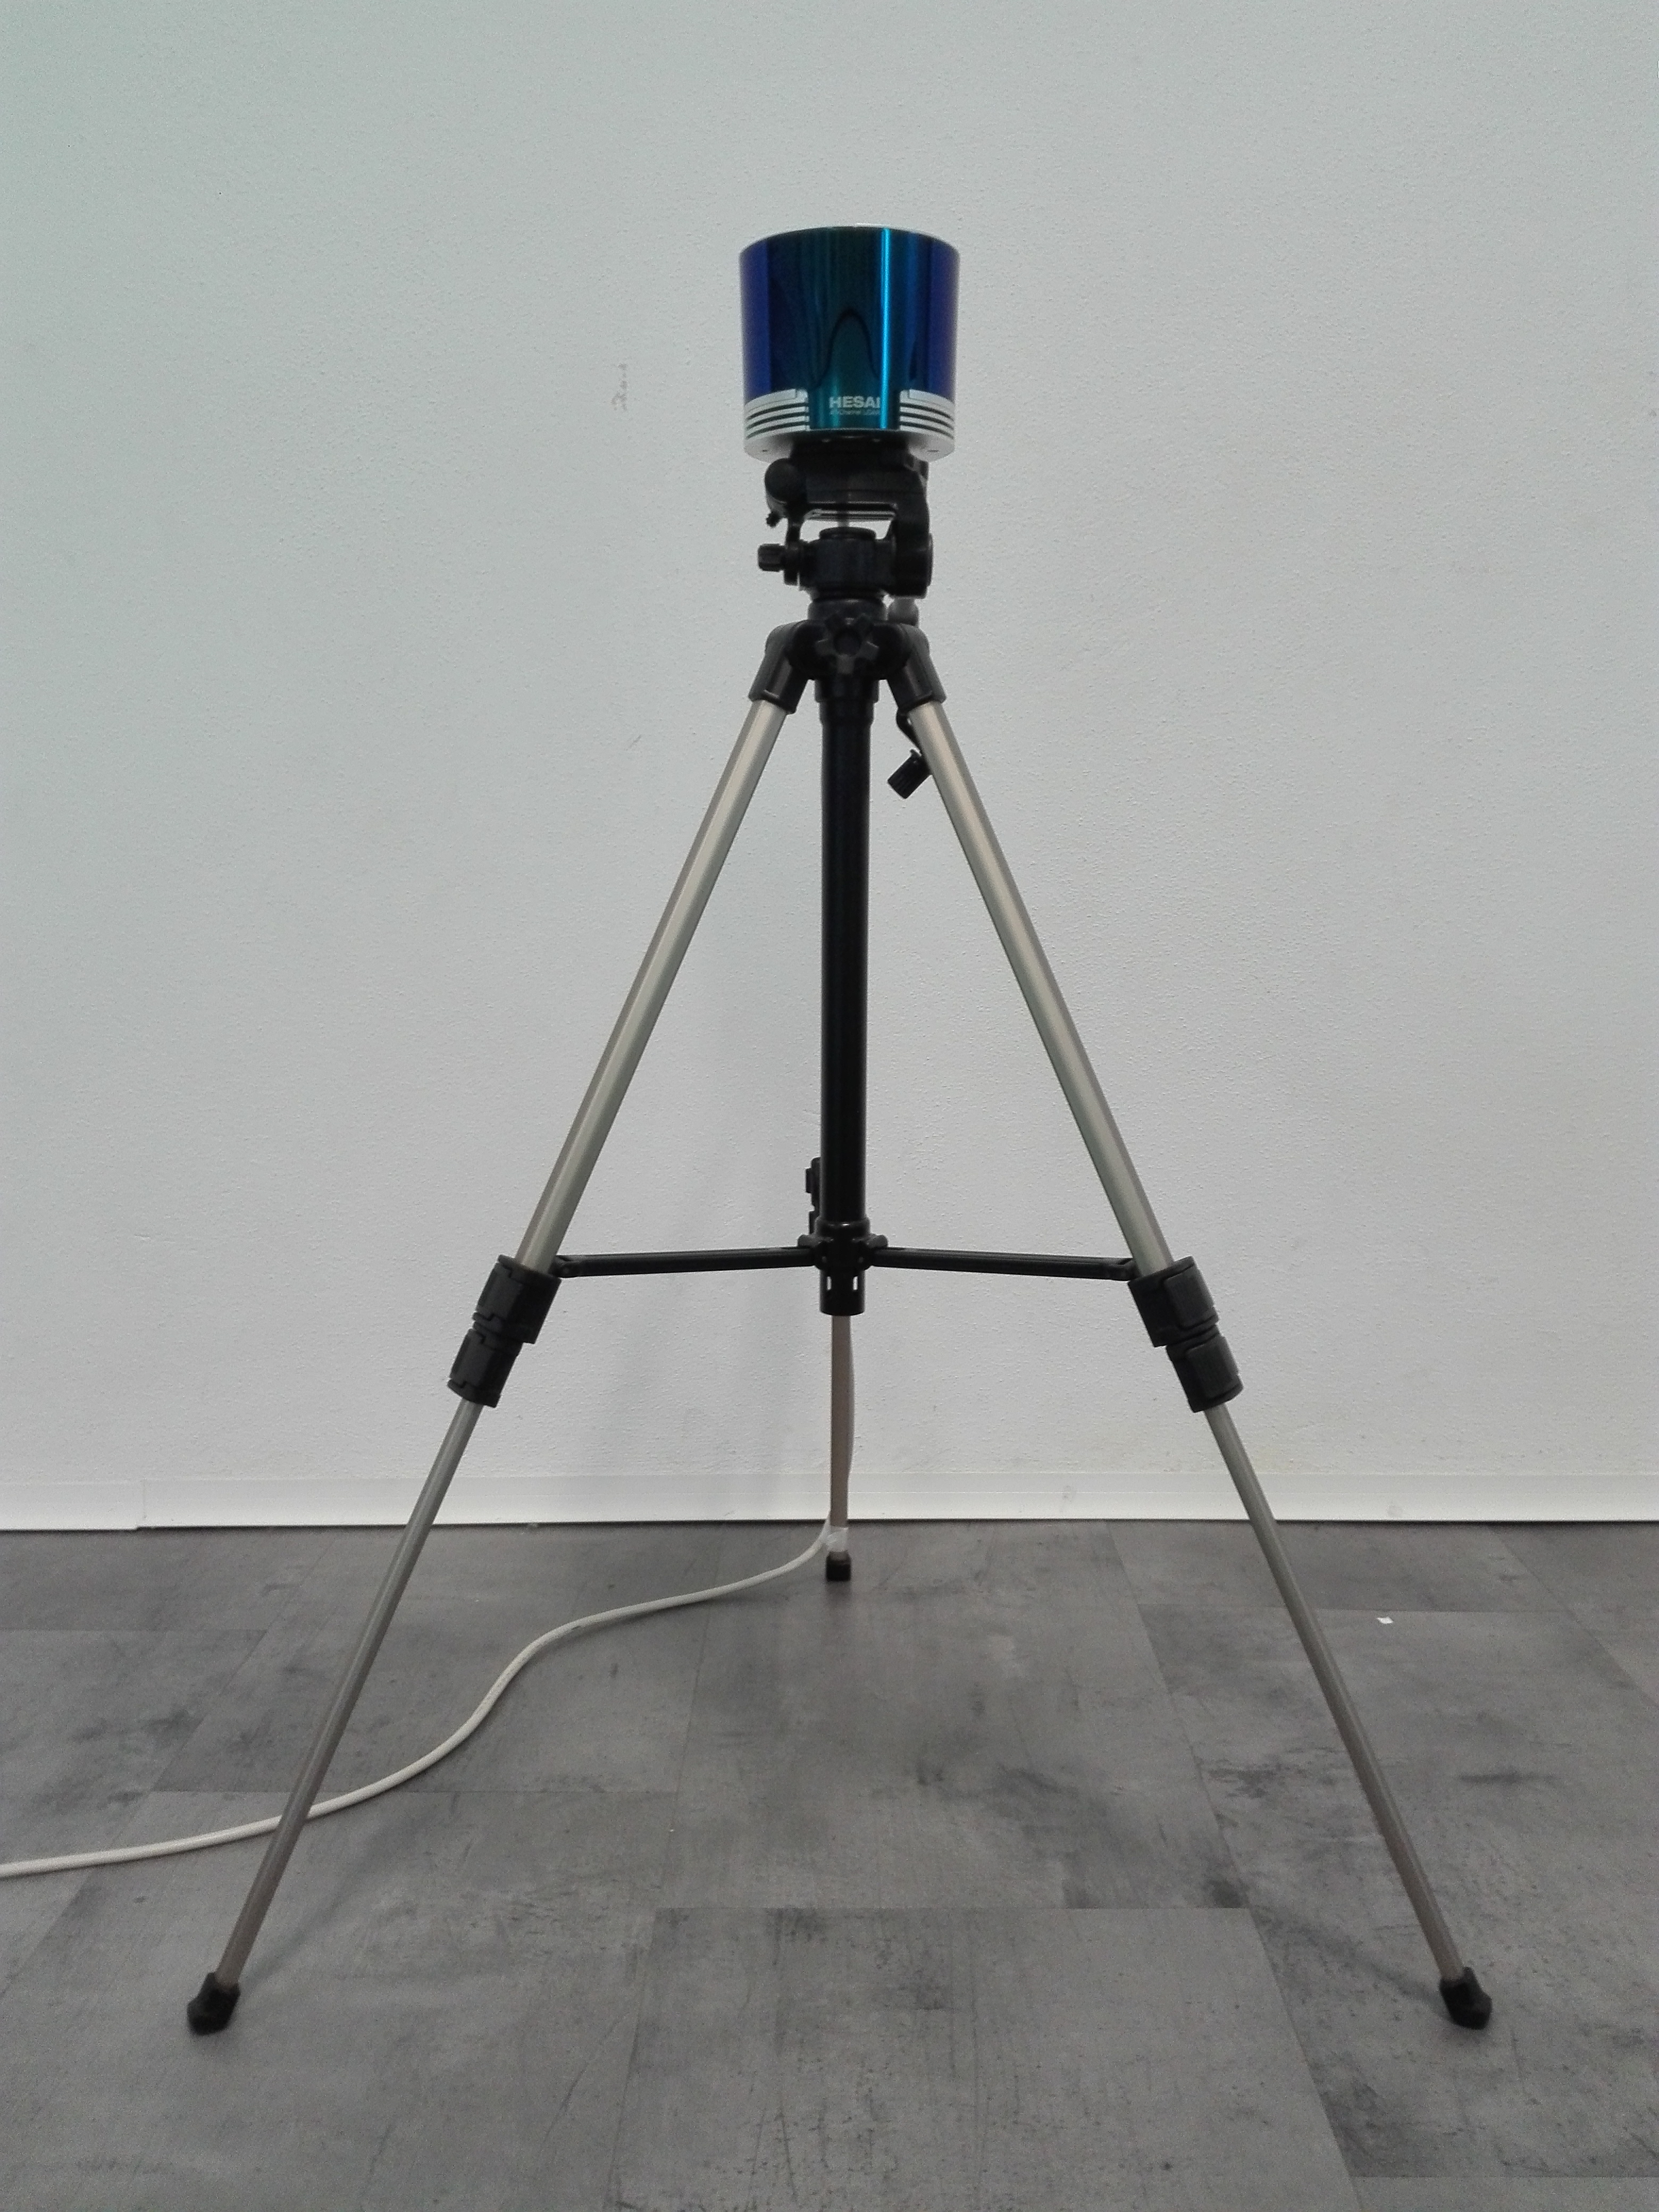
\includegraphics[width=0.4\textwidth]{img/experimental-setup/pandar40-on-tripod.jpg}
	\caption{HESAI Pandar40 \ac{lidar} on a Velbon CX-460 tripod.}
	\label{fig:pandar40-on-tripod}
\end{figure}

Despite the two \acp{lidar}'s laser nominal frequencies not being equal, no majors drawbacks are expected due to the mismatch. Velodyne's VLP-16, the victim, operates at \SI{903}{\nano\meter} and HESAI Pandar40, the interferer, operates at \SI{905}{\nano\meter}. Ideally, the same \ac{lidar} model would be used for the victim and interferer, but such material was not available. Nevertheless, we are unable to predict how the different number of channels, asymmetric channel distribution, variable angular step and different laser wavelength will impact the interference behaviour, due to the lacking of prior knowledge available on the area.

\subsection{Experimental Test Scenarios}
\label{subsec:lidar-interference:test-scenarios}

Two places were used as test scenarios for \ac{lidar} interference: Aveiro's \ac{it} Dark Room and \ac{irislab} \ac{msl} robotic soccer field. On the former, acquaintance with the experimental setup, calibration procedures and tests to gathered preliminary knowledge on \ac{lidar} interference were carried. On the latter, experimental tests were devised to research the impact of relevant parameters under study on \ac{lidar} interference. 

Aveiro's \ac{it} Dark Room is an optical laboratory that is capable of blocking all external light (hence its name). It measures $\SI{5.20}{\meter} \times \SI{6.97}{\meter} \times \SI{2.80}{\meter}$ and is equipped with desks, chairs, optical experimental setups, among other things, creating a noisy scenario for a \ac{lidar} rangefinder. 
\ac{irislab} \ac{msl} robotic soccer field measures $\SI{18.0}{\meter} \times \SI{11.5}{\meter}$ and is placed inside \ac{irislab} building, a research facility whose main division has $\SI{34.346}{\meter} \times \SI{16.097}{\meter} \times \SI{4.289}{\meter}$, if measured to the ceiling and not the ceiling girders. 

All distance measures presented on this Chapter are taken using LOMVUM LV66V \SI{80}{\meter} laser rangefinder. When taking measures, the orientation of the rangefinder was kept in the interval of $[\SI{-0.2}{\degree}, \SI{0.3}{\degree}]$. The error associated to each laser measurement, according to LOMVUM datasheet\footnote{No online manual was found. Measurement error determined by consulting the product printed datasheet, supplied with the device.} is \SI{1.5}{\milli\meter}. To minimize the error introduced by the human operator, 10 measurements were done and their average was taken, considering it the value that is represented, using the LOMVUM's laser rangefinder capabilities.


\subsection{Parameters under study}
On \ac{irislab}, several tests were devised to tackle the problem of \ac{lidar} interference from different perspectives. Tests scenarios were carried, where only one parameter is varied, in an attempt to understand the interference behavior between data. The test parameters under studied, from which different datasets were recorded are:

\begin{itemize}
	\item \textbf{Distance:} Keeping the \acp{lidar} azimuthal origin aligned and with their focal center at the same height, the distance between the interferer and victim is changed, by moving the interferer further away. The distance between the two was varied in steps of \SI{1}{\meter}, from \SIrange{1}{12}{\meter};
	\item \textbf{Height:} For a fixed distance between the two \acp{lidar}, with its azimuthal origin aligned, the height between the two is varied in non-uniform steps, from \SIrange{0.623}{1.277}{\meter} measured in relation to the floor, which results in \SIrange{-0.295}{0.359}{\meter} when compared with the victim \ac{lidar} height;
	\item \textbf{\acp{lidar} \ac{los} obstruction:} To quantify the impact of direct and indirect interference, an obstacle is placed on the \acp{lidar} \ac{fov}, breaking the \ac{los} between the two \acp{lidar} This test scenario places the interferer at the even distances from the distance test, with the obstacle placed at the middle distance between the victim and interferer \ac{lidar}. The remaining test conditions are similar to the Distance tests;
	\item \textbf{Rotation Speed:} To measure the impact of different rotation speeds between the \acp{lidar}, the victim's \ac{lidar} is kept at the same rotation speed as the other tests, while the interferer \ac{lidar} rotation speed is changed. Distance is constant, the \ac{lidar}'s azimuthal origin is aligned and their focal length is at the same height;
	\item \textbf{Orientation:} To study the interference directionality, the relative angular position between the victim's and the interferer \ac{lidar} is changed, while keeping their focal length at the same height and the same distance for all variations of this parameter.
\end{itemize}


\subsection{Dataset Organization}
A thesis objective on its own (see Section~\ref{sec:introdcution:objectives}), dataset organization is a crucial for a proper data analysis. With 5 parameters under test, each with several values, 60 different interference test exists, in addition to camera calibration data and data without interference. On total, more than \SI{600}{\giga\byte} of pre-processed raw data, ready to be analyzed, is stored, in a total of almost 180 \ac{ros} bag files, totalling almost 4 hours and 20 minutes of playable data. Several hundred files, among camera calibration, rigid body transform and results, are also contained on the dataset structure, for a total of more than \SI{1}{\tera\byte} of data and results.

A comprehensive diagram that details the dataset directory and file tree hierarchy for data recording is given on~\nameref{appendix:datasets-tree}. The \textit{Experimental Datasets} folder is the root folder of the data, containing the two test locations, \textit{IRIS Laboratory} and \textit{IT2 Dark Room}. 

The standardization of tests scenarios started on \ac{it} 2 Dark Room, but only matured on \ac{irislab}. This standardization forces guidelines on file and folder naming, directory structure organization and data to record. On every folder, a \textit{README.md} file is present, detailing the files and/or folders in its hierarchy level, and the test conditions, if applicable. 

On \ac{it} 2 Dark Room, only \textit{Scenario B} follows these guidelines, which were inspired by \ac{kitti}'s dataset~\cite{Geiger2013a}. Since our setups location is fixed, each location defines a root folder for all the tests happening in that location, with its subfolders being the day on which the data was acquired. These type of folders contain  3 subfolders, whose goal is detailed below and an extract of its  hierarchy organization is given on figure~\ref{fig:test-subfolders}.

\begin{figure}[H]
	\centering
	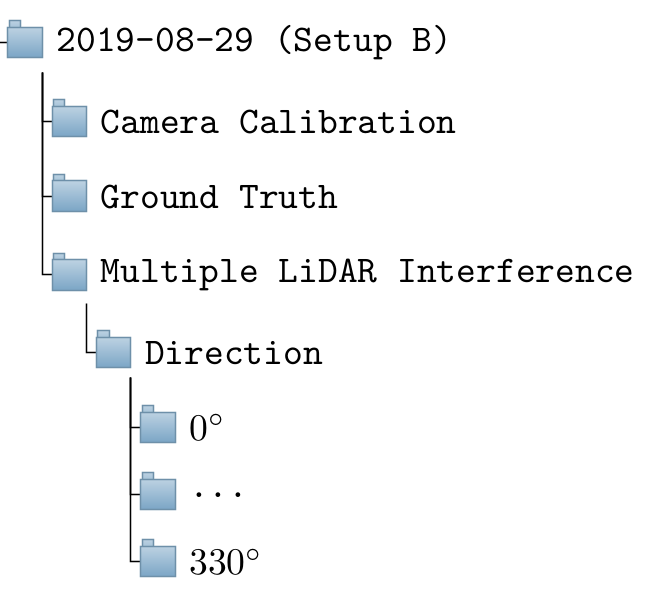
\includegraphics[scale=0.3]{img/datasets/test-subfolders.png}
	\caption{Detail of the hierarchy of a ``test day''. On each day data was recorded, calibration and ground-truth data were recorded. \textit{Multiple Lidar Interference} folder contains the parameters under test and each of the tested values.}
	\label{fig:test-subfolders}
\end{figure}


\begin{enumerate}
	\item \textit{Camera Calibration}: Contains the calibration images, intrinsic calibration parameters, \ac{ros} bag files containing the camera and \ac{lidar} raw and pre-processed data and the log file of the calibration procedure;
	\item \textit{Ground Truth}: One or more \ac{ros} bag file containing the static scenario, without objects of interest placed on the camera's and \ac{lidar} \ac{fov} and without \ac{lidar} interference;
	\item \textit{Multiple LiDAR Interference}: This folder contains a series of subfolders, each for a parameter under test. For each parameter under test folder, subfolders contain the data and results for each of the value that the parameters takes.
\end{enumerate}

On a specific value for a parameter under test, three bag files are present, as shown in figure~\ref{fig:parameter-test-files}. \textit{interference.bag} is a pre-processed \ac{ros} bag file that contains only \ac{lidar} data with interference. This pre-processing consists on cropping the \textit{original\_raw.bag} file to remove the initial seconds (from \SIrange{20}{30}{\second}), when the interferer \ac{lidar} is still booting up. \textit{ground\_truth} corresponds to data recorded under the conditions of \textit{interference.bag}, but without interference, i.e., the interferer \ac{lidar} is its position for the test, but switched off.

\begin{figure}[H]
	\centering
	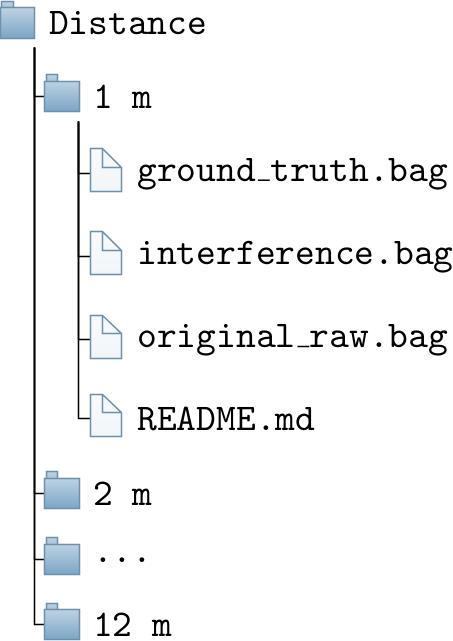
\includegraphics[scale=0.3]{img/datasets/parameter-test-files.png}
	\caption{Data recorded using \texttt{rosbag} tool, for a single value of a parameter under test. \textit{README.md}, on this type of folder, details the conditions under which data was gathered.}
	\label{fig:parameter-test-files}
\end{figure}


On \textit{IRIS Laboratory} folder, two test folders are present, containing all the data gathered on \ac{irislab}, \textit{2019-08-28} and \textit{2019-08-29}. For each of the folders, different calibration parameters are available, along with ground truths and calibration data. For \textit{\ac{it} 2 Dark Room}, only the data on the folder \textit{2019-07-31} is relevant to interference analysis.

To ease the access to this data structure, \texttt{datasets\_path} library was implemented, both on C++ and Python 3, to allow ubiquitous managing of data loading for tests and saving of results.

\section{Bosch\cp~Dataset}
We start by investigating \ac{lidar} interference using Bosch's dataset. This dataset consists of 3 \ac{ros} bag files, one recorded by a HESAI Pandar40 and two other by Velodyne's VLP-16. Each of the bag files correspond to the same experimental scenario: the two \acp{lidar} are placed, side by side, on top of a table, with the Pandar40 about \SI{50}{\centi\meter} to the left of the VLP-16. For each of the tests, data is recorded for about \SIrange{10}{15}{\second} and the two \acp{lidar} are always switched on.

To analyse the interference, we start by analysing at the data in \texttt{Rviz}, noticing two phenomenons: 

\begin{enumerate}
	\item Data appears to be more noisy, as if it was oscillating with greater magnitude around a fixed point on its measurement axis, when comparing with \ac{kitti}'s dataset;
	\item Some of the measurements correspond to points outside of the room dimensions.
\end{enumerate}

For the first case, we present two hypotheses: it is caused by the interference of the other \ac{lidar} or due to the measurements being taken in small rooms. The understand the second phenomenon, a two dimensional scatter map of the point cloud, viewed from above, is plotted. This representation does not take in consideration the measurement density, which might be misleading, since interfered measurements should have a higher ``geometric'' dispersion when comparing with the correct measurements of the real world.

These results are present on figure~\ref{fig:bosch-pandar-vs-vlp16}, with the left subfigure, (\subref{fig:bosch-pandar40}), showing HESAI's Pandar40 data, represented in green, and the right subfigure, (\subref{fig:bosch-vlp16-1}), showing Velodyne's VLP-16 data, represented in yellow. For each of the subfigures, we notice in the center a rectangular shape, the room, and the outliers are distributed in a circular arrange, with preference for some azimuthal angles. The circular range is due to the hardware time window to measure the reception pulse and software distance threshold to register the data. On Pandar40, the software constrain is \SI{200}{\meter} and on VLP-16 is \SI{130}{\meter}. 

Considering the HESAI's \ac{lidar} is left to the Velodyne's \ac{lidar}, the occurrence of interference seem to be more significant to HESAI's right, i.e., between the two \acp{lidar}. On the other hand, Velodyne's outliers tend to its left, the side on which the HESAI's is in. With HESAI's outliers concentrated on its first geometric quadrant and Velodyne's outliers on the second geometric quadrant, such results seem to indicate that interference is directional. However, from this data we cannot determine if this is due to direct interference, reflections or both.

\begin{figure}[ht!]
	\centering
	\begin{subfigure}[t]{0.45\textwidth}
		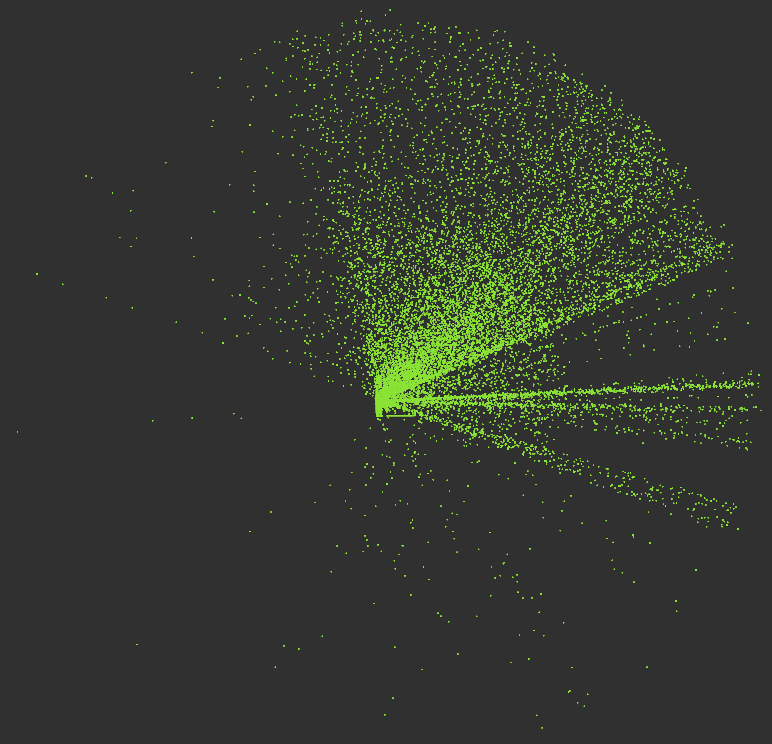
\includegraphics[width=\textwidth]{img/bosch/pandar40.png}
		\caption{HESAI's Pandar40 data scatter plot.}
		\label{fig:bosch-pandar40}
	\end{subfigure}
	\qquad
	\begin{subfigure}[t]{0.45\textwidth}
		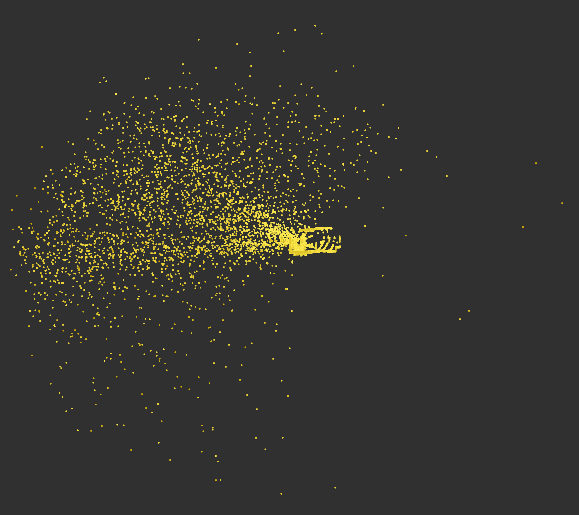
\includegraphics[width=\textwidth]{img/bosch/vlp16-test1.png}
		\caption{Velodyne's VLP-16 data scatter plot}
		\label{fig:bosch-vlp16-1}
	\end{subfigure}
	\caption{Scatter plot of the data gathered by HESAI's Pandar40, (\subref{fig:bosch-pandar40}), and Velodyne's VLP-16, (\subref{fig:bosch-vlp16-1}). The measurements are plotted only on the X-Y plane, flatenning the height of the points. }
	\label{fig:bosch-pandar-vs-vlp16}
\end{figure}

We also analyze the results from the second VLP-16bag file, and compare with the first, on figure~\ref{fig:bosch-vlp16-comparison}. The previous shown data, on figure~\ref{fig:bosch-vlp16-1} is shown in yellow and the second dataset in blue. On the center, the room can be seen, and the data, independently of the bag file, seems to have the same dispersion and directionality.

\begin{figure}[ht!]
	\centering
	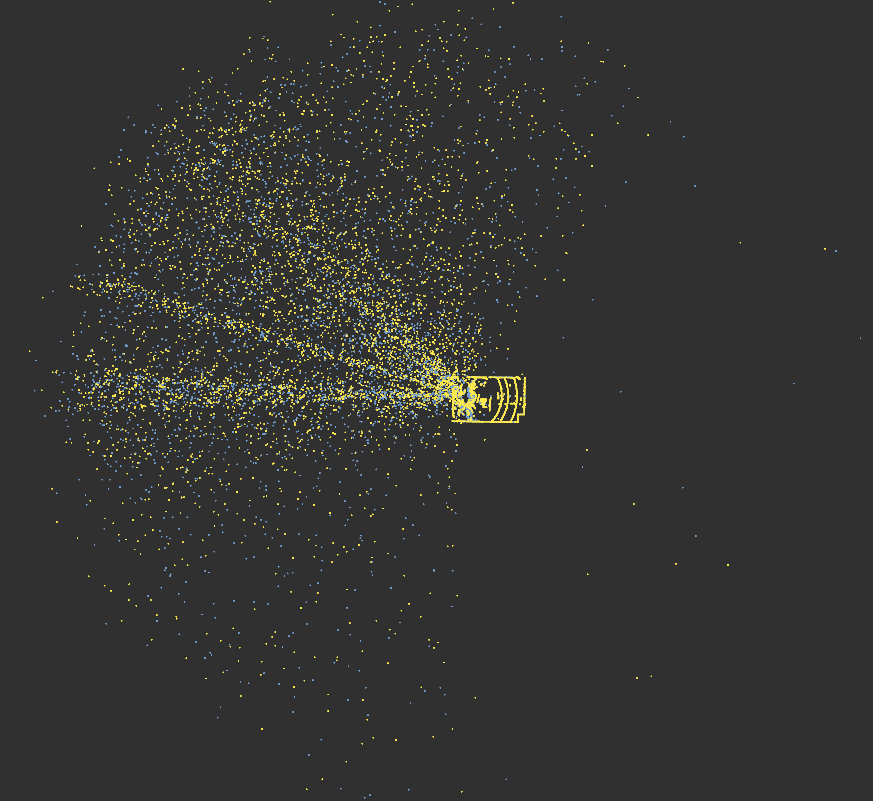
\includegraphics[scale=0.33]{img/bosch/vlp16-tests-overlaid.png}
	\caption{Scatter plot of the \ac{ros} bags containing Velodyne's VLP-16 data, gathered under the same conditions with almost an hour of difference. Thee measurements are plotted only on the X-Y plane, flatenning the height of the points. Comparison between the grid and blue points shows a macro-correspondance }
	\label{fig:bosch-vlp16-comparison}
\end{figure}

Since the room had people moving and no data without interference is present, this dataset cannot be used for a refined analysis of the interference, since the approach and methods we devise suppose that the environment is static, in order for a ground truth model to be generated. Since we have no camera information, no object detection processing chain can be implemented (similar to Chapter~\ref{chapter:object-detection}). 

Our solution is then to quantize this outliers and trying to understand more about their behavior, which is the approach detailed on the next Section.


\section{Room Outliers Contabilization}
After the qualitative analysis of the previous Section on Bosch's dataset, from which we concluded that the \ac{lidar} interference appears to be directional and causes outliers outside of the room dimensions, this Section details the implementation and results of a quantitative approach to the events described on phenomenon 2: \ac{lidar} measurements outside room dimensions.

To analyze the data, a \ac{ros} node, with both offline and online versions, was implemented. Offline operation implies that the node does not have real-time constraints, being capable of handling large \ac{ros} bag files and datasets. The main difference from the online operation, that as been used so far, is that the node does not require another node on the network to publish data for him (tipically, a \ac{ros} bag player or a device driver). Instead, the node loads and parses the bag file, as fast as it can or as fast is instructed to, keeping its data private on its own program memory. This alternative permits processing large amounts of data and realizing complex analysis on it.

To quantify this inteference, the node only requires knwoledge about the room dimensions and it  determines the number of messages received, average points per message, absolute and relative number of outliers and inliers. Despite not accounting for interference inside the room dimensions, this interference model intends to measure what, to the ``naked eye'', is clearly and erroneous measure, caused by interference: measurements outside the physical dimensions of the room where the \acp{lidar} are located. Since the possible interference inside the room dimensions is not considered, we can view this metric as a minorant for the \ac{lidar} interference.
%, which can never be confused with other \ac{lidar} behaviors and noise.

\subsection{Bosch Dataset}

\subsection{Our Experimental Dataset}

\subsubsection{Distance}
\subsubsection{Height}
\subsubsection{\acp{lidar} \ac{los} Obstruction}
\subsubsection{Direction}


\section{Ground-Truth Generation}
\label{sec:lidar-interference:ground-truth}

\subsection{Frame Stitching}
\label{subsec:lidar-interference:frame-stitching}
	
\subsection{Frame Accumulation}
\label{subsec:lidar-interference:frame-accumulation}

\subsection{Comparison}

%Direct interference (on Kim's experimental setup and hardware) is likely to saturate the receptor of the interfered \ac{lidar}, which may or may not be considered a valid measurement by the hardware and may discarded by the driver before being registered;

\section{Voxel-ize Analysis}
\subsection{Theoretical Principle}
\subsection{Implementation}
\subsection{Results}
\subsubsection{Distance}
\subsubsection{Height}
\subsubsection{\acp{lidar} \ac{los} Obstruction}
\subsubsection{Direction}

\section{Point-to-Point Analysis}
\subsection{Theoretical Principle}
\subsection{Implementation}
\subsection{Results}
\subsubsection{Distance}
\subsubsection{Height}
\subsubsection{\acp{lidar} \ac{los} Obstruction}
\subsubsection{Direction}

\section{Interference on \acp{roi}}

\section{\acl{sota} Comparison}
